%====================================================================================
\section[Ejemplo \emph{Free rider}]{Ejemplo del comportamiento \emph{Free rider}}
%====================================================================================

\begin{frame}{Ejemplo del comportamiento \emph{Free rider} (=gorrón = polizón)}
	\begin{multicols}{2}
		\begin{itemize}
			\item Supongamos que cuesta \$4 proporcionar limpieza a la calle frente a mi casa.
			\item Yo o mi vecino podemos pagar por ello.
			\item Ambos valoramos las calles limpias en \$3.
			\item Si uno de los dos paga \$4, el otro está  mejor.
		\end{itemize}
	
		\begin{center}
			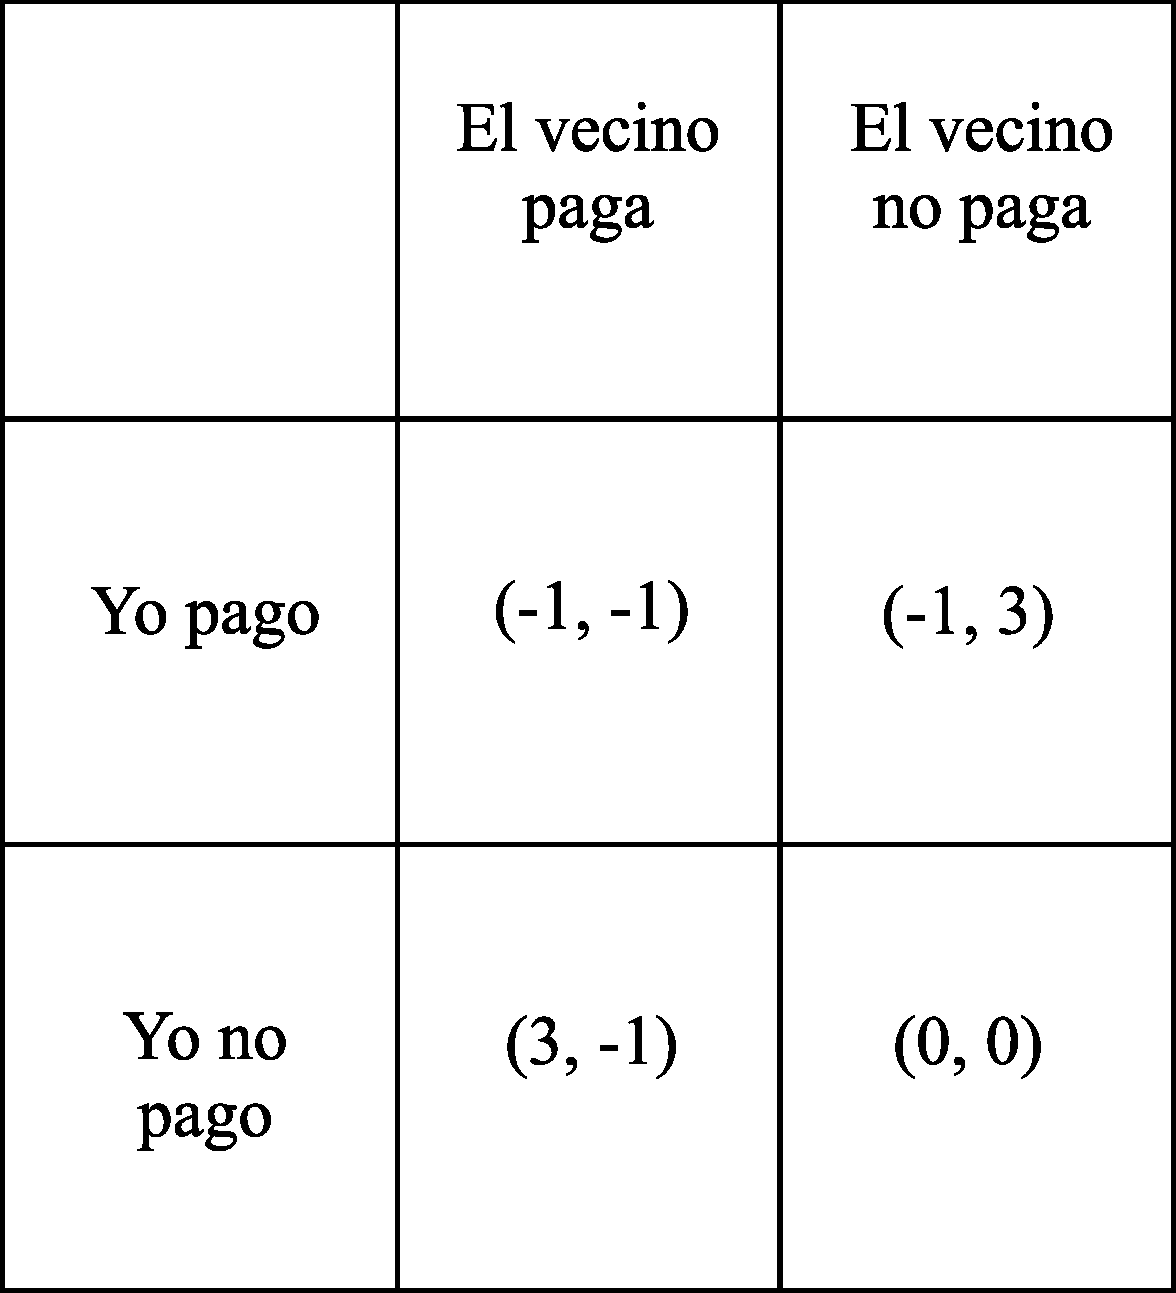
\includegraphics[width = 0.9\linewidth]{figures/fig_12.pdf}
		\end{center}
	\end{multicols}
	
	Estrategia dominante = nadie paga, pero es ineficiente (no max $\sum$ pagos netos). Se max $\sum$ papos netos si solo uno paga
\end{frame}